% The twisted frame: an explanation for non-specialists (study 1 of the D4 code-switching project).
% Compile with pdfLaTeX (e.g. on Overleaf); only standard packages are used.
% Japanese companion: twisted_frame解説.md (same content without figures).
% The formal statement and proof are the Proposition of 論文草稿/研究1_原稿_v12/main_v12.tex (Sec. 4).
\documentclass[11pt,a4paper]{article}
\usepackage[margin=25mm]{geometry}
\usepackage{amsmath,amssymb,amsthm}
\usepackage{booktabs}
\usepackage{array}
\usepackage{tikz}
\usetikzlibrary{arrows.meta,positioning,calc,decorations.pathreplacing}
\usepackage[colorlinks,linkcolor=blue!50!black,citecolor=blue!50!black,urlcolor=blue!50!black]{hyperref}

\newcommand{\GF}{\mathrm{GF}(2)}
\newcommand{\ind}{\mathbf{1}}
\providecommand{\ket}[1]{\ensuremath{|#1\rangle}}
\newtheorem*{prop}{Proposition}

\title{The twisted frame:\\ tracking the measurements of the $\mathbb{D}_4$ code exactly and fast}
\author{Study 1 of the $\mathbb{D}_4$ code-switching project (explanatory note)}
\date{12 November 2026}

\begin{document}
\maketitle

\begin{abstract}
To estimate the error threshold of the $\mathbb{D}_4$ Clifford-hierarchy stabilizer code we must simulate, many times, how a noisy code state responds to the measurement of its checks. The checks are not Pauli operators, they stop commuting when an error is present, and the quantum state is far too large to store. This note explains, for readers without a background in quantum error correction, the representation we use instead. The state is written as a set of bit strings that solves a system of linear equations modulo 2, carrying a sign given by a quadratic function, on top of a fixed cubic sign that never has to be computed. Every noise event and every measurement keeps this form, so the state can be followed exactly with small binary matrices. We call it the \emph{twisted frame}; the name is ours, not an established term. We explain why it is valid for the memory experiment of study~1 and why it is the right tool there.
\end{abstract}

\section*{The idea in one sentence}
However many errors and measurements occur, the state of the $\mathbb{D}_4$ code always has the form
\begin{center}
\emph{(solutions of a linear system mod 2)} \;$\times$\; \emph{(sign of a quadratic function)} \;$\times$\; \emph{(a fixed cubic sign)},
\end{center}
and only the first two factors ever change.

\section{What we need to compute}

Study~1 simulates a \emph{memory experiment}. A logical state is encoded in the code, and then, round after round, (1) random errors hit the physical qubits, (2) the checks (stabilizers) of the code are measured to obtain a syndrome, and (3) a decoder infers and corrects the errors. At the end we ask whether the logical information survived. Repeating this $10^5$ times for several system sizes $L$ and error rates $p$ gives failure-rate curves whose crossings estimate the threshold. The tool we need answers one question exactly: \emph{for a given realisation of the noise, which measurement outcomes occur, and with what probabilities?}

\subsection{Why the standard tools fail}
\begin{itemize}
\item \textbf{Store the state vector.} The $L\times L$ torus has $n=9L^2$ qubits, i.e.\ $2^n$ amplitudes ($2^{81}$ at $L=3$). Restricting to error-free configurations still leaves $2^{27}\approx1.3\times10^8$ amplitudes at $L=3$ and $2^{75}$ at $L=5$.
\item \textbf{Stabilizer simulators} such as Stim require every check to be a product of Pauli operators. The $X$-type checks of the $\mathbb{D}_4$ code are Pauli operators multiplied by controlled-$Z$ (CZ) gates, and measuring them needs CCZ gates.
\item \textbf{The surrogate of the previous study} replaced the checks by plain Pauli checks and added independent noise for the CZ factors. It cannot reproduce the non-commutativity described next.
\end{itemize}

\subsection{What makes the \texorpdfstring{$\mathbb{D}_4$}{D4} code hard}
\begin{itemize}
\item \textbf{The checks carry CZ gates.} The check of colour $c$ at vertex $v$ is $S=X^{s}(-1)^{q(a)}$: $X^{s}$ flips six qubits and $(-1)^{q(a)}$ is the sign produced by two CZ gates, so $q$ is a sum of products of two bits (a quadratic function).
\item \textbf{Errors make the checks non-commuting.} Without errors all checks commute. An $X$ error creates a \emph{flux}, and then some checks of different colours anticommute: measuring a check $S_1$, then $S_2$, then $S_1$ again reproduces the first outcome of $S_1$ only with probability $1/2$. Outcomes are random, and the syndrome is no longer a fixed function of the errors.
\item \textbf{Corrected errors can leave a CZ-type residue.} Even after a flux has been corrected, the state can carry a CZ-type error that randomises checks of other colours.
\end{itemize}

\section{Bits, flat configurations and the code state}

A computational-basis state $\ket{a}$ is a bit string $a\in\GF^n$. In the $\mathbb{D}_4$ code the qubits sit on the edges of the lattice, three colours per edge, so $a$ assigns a bit to every edge and colour (a \emph{gauge configuration}). A configuration is \emph{flat} if, for every triangle and colour, the three edge bits add up to $0$ modulo $2$; a triangle where they add up to $1$ carries a flux. The $Z$-type checks measure exactly these sums.

The error-free code state is
\begin{equation}
\ket{\psi_0}=\sum_{b\in C_0}(-1)^{\phi_0(b)}\ket{b},
\label{eq:code}
\end{equation}
where $C_0$ is the set of flat configurations (in the logical sectors we track) and $\phi_0$ is a \emph{cubic} function built from products of one bit of each colour. This cubic sign is the ``twist'' of the twisted gauge theory; the toric code would have no sign at all.

Flatness is a set of linear equations, so $C_0$ is the solution set of a linear system: every $b\in C_0$ can be written as $b=Mt$ with a short coordinate vector $t\in\GF^k$ (one bit per vertex and colour, plus one winding bit per logical colour; $k=3L^2$). At $L=9$, $k=243$, which is tiny compared with $2^{729}$ amplitudes.

\paragraph{The fact behind fast Clifford simulators.} Every stabilizer state (any state a Clifford circuit can prepare) has the form $\psi(a)\propto i^{\ell(a)}(-1)^{Q(a)}\ind[a\in\mathcal{A}]$ with $\mathcal{A}$ an affine subspace and $Q$ quadratic (Dehaene--De Moor). That is why Stim-like simulators are fast. Because of the cubic sign $\phi_0$, code states of the $\mathbb{D}_4$ code are \emph{not} stabilizer states. The twisted frame shows that this does not matter.

\section{The representation}

\begin{prop}[Sec.~4 of the study-1 manuscript]
Starting from $\ket{\psi_0}$ and applying any sequence of Pauli operators, CZ gates, measurements of $Z$-type checks and projective measurements of the dressed $X$-type checks (possibly multiplied by a Pauli $Z$), the state is, up to normalisation,
\begin{equation}
\psi(a)=(-1)^{\phi_0(b)+Q(b)}\,\ind[b\in B],\qquad b=a+x,
\label{eq:tf}
\end{equation}
where $x\in\GF^n$ is the accumulated $X$ frame, $B\subseteq C_0$ is an affine subspace and $Q$ is a quadratic form over $\GF$. Every measurement outcome has probability $0$, $\tfrac12$ or $1$.
\end{prop}

\begin{figure}[t]
\centering
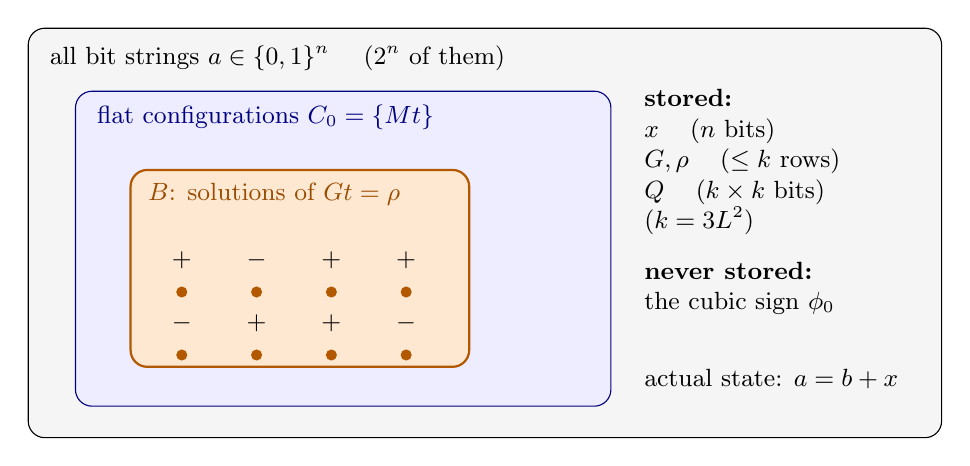
\begin{tikzpicture}[font=\small]
  \draw[rounded corners=6pt, fill=gray!8] (0,0) rectangle (11.6,5.2);
  \node[anchor=north west] at (0.15,5.1) {all bit strings $a\in\{0,1\}^n$ \quad ($2^n$ of them)};
  \draw[rounded corners=6pt, fill=blue!7, draw=blue!50!black] (0.6,0.4) rectangle (7.4,4.4);
  \node[anchor=north west, blue!50!black] at (0.75,4.35) {flat configurations $C_0=\{Mt\}$};
  \draw[rounded corners=6pt, fill=orange!18, draw=orange!70!black, thick] (1.3,0.9) rectangle (5.6,3.4);
  \node[anchor=north west, orange!60!black] at (1.4,3.35) {$B$: solutions of $Gt=\rho$};
  \foreach \i/\s in {0/+,1/-,2/+,3/+} {
    \node at (1.95+0.95*\i,2.25) {$\s$};
    \fill[orange!70!black] (1.95+0.95*\i,1.85) circle (2pt);
  }
  \foreach \i/\s in {0/-,1/+,2/+,3/-} {
    \node at (1.95+0.95*\i,1.45) {$\s$};
    \fill[orange!70!black] (1.95+0.95*\i,1.05) circle (2pt);
  }
  \node[align=left, anchor=west] at (7.7,3.5) {\textbf{stored:}\\ $x$ \;\; ($n$ bits)\\ $G,\rho$ \;\; ($\le k$ rows)\\ $Q$ \;\; ($k\times k$ bits)\\ ($k=3L^2$)};
  \node[align=left, anchor=west] at (7.7,1.9) {\textbf{never stored:}\\ the cubic sign $\phi_0$};
  \node[align=left, anchor=west] at (7.7,0.75) {actual state: $a=b+x$};
\end{tikzpicture}
\caption{The twisted frame. The amplitude is non-zero only on the set $B$ (orange) of flat configurations, shifted by the $X$ frame $x$. On $B$ the amplitude is $\pm1$; the sign is the fixed cubic sign $(-1)^{\phi_0}$ times the quadratic sign $(-1)^Q$ (the $\pm$ marks illustrate the latter). Only $x$, the linear system $Gt=\rho$ that defines $B$, and $Q$ are stored.}
\label{fig:rep}
\end{figure}

The three stored ingredients are (Fig.~\ref{fig:rep}):
\begin{center}
\begin{tabular}{>{\raggedright}p{0.17\linewidth}>{\raggedright}p{0.48\linewidth}p{0.25\linewidth}}
\toprule
ingredient & meaning & storage \\
\midrule
$X$ frame $x$ & all $X$ errors and $X$ corrections so far; we look at the state ``through'' this shift & $n$ bits \\
$B$ & the flat configurations present in the superposition (an affine subspace of $C_0$) & a row-reduced linear system, at most $k$ rows \\
$Q$ & signs acquired from noise and measurements; a \emph{quadratic} form & $k\times k$ bits plus a linear part \\
$\phi_0$ & the cubic sign of the initial code state & \emph{not stored} \\
\bottomrule
\end{tabular}
\end{center}
The name: \emph{twisted} refers to the cubic sign $\phi_0$ of the twisted gauge theory, \emph{frame} to the Pauli frame $x$ familiar from stabilizer simulators.

\paragraph{Why $\phi_0$ is never needed.} A check $S$ leaves the code state unchanged, $S\ket{\psi_0}=\ket{\psi_0}$. Written configuration by configuration this means that for every flat $b$
\begin{equation}
\phi_0(b+s)+\phi_0(b)=q(b+s),
\label{eq:identity}
\end{equation}
where $s$ marks the qubits flipped by the check and $q$ is the quadratic function of its CZ gates. The simulation only ever needs the \emph{ratio} of the amplitudes at $b$ and $b+s$, i.e.\ a \emph{difference} of $\phi_0$, and Eq.~\eqref{eq:identity} replaces that difference by the quadratic $q$.

\section{How each operation updates the state}

\begin{center}
\begin{tabular}{>{\raggedright}p{0.28\linewidth}>{\raggedright}p{0.4\linewidth}p{0.22\linewidth}}
\toprule
operation & update & cost \\
\midrule
$X$ error or $X$ correction & flip a bit of $x$ & one bit \\
$Z$ error & add a linear term to $Q$ (multiply by $(-1)^{a_q}$) & one row XOR \\
CZ (e.g.\ a circuit fault) & add a quadratic term to $Q$ (multiply by $(-1)^{a_ia_j}$) & two rows and columns \\
$Z$-type check & outcome read from $x$ ($B$ is flat, so every flux lives in $x$) & three bits \\
dressed $X$-type check & one of the two cases below & a few matrix rows \\
\bottomrule
\end{tabular}
\end{center}

\subsection{Measuring a dressed check: two cases}

To measure $S=X^s(-1)^q$ we first form the \emph{affine} function
\begin{equation}
f(b)=q(b+s+x)+q(b+s)+Q(b+s)+Q(b),
\label{eq:f}
\end{equation}
the sign of the ratio of $S\psi$ to $\psi$ at $b$. It is affine because $q$ and $Q$ are quadratic and we take a difference. The part $q(b+s+x)+q(b+s)$ is the $Z$-type effect produced when the $X$ frame meets a CZ gate (the ``Pauli dressing''); CZ-type residues enter here as well.

\begin{figure}[t]
\centering
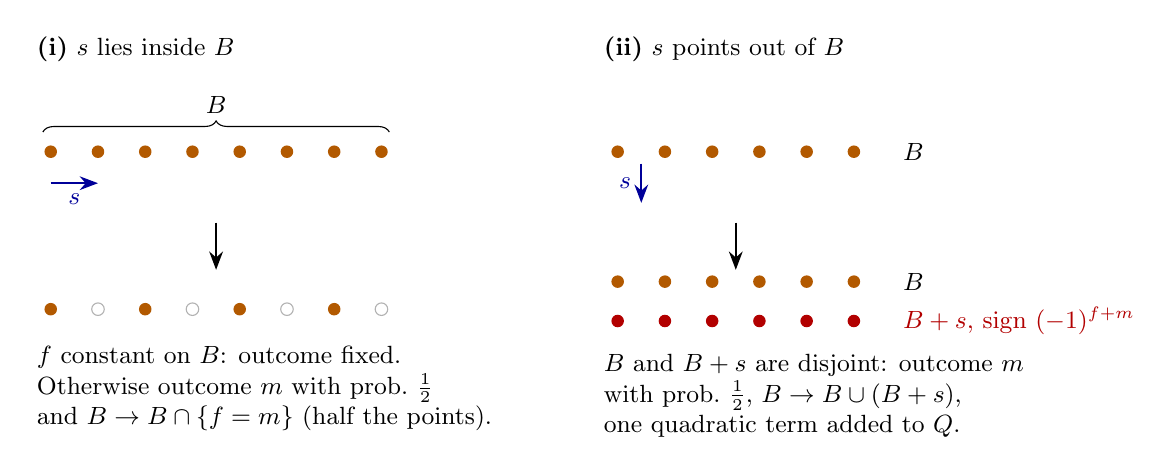
\begin{tikzpicture}[font=\small, dot/.style={circle, fill=orange!70!black, inner sep=1.6pt}, gone/.style={circle, draw=gray!60, inner sep=1.6pt}]
  % case (i)
  \node[anchor=west] at (-0.3,3.9) {\textbf{(i)} $s$ lies inside $B$};
  \foreach \i in {0,...,7} { \node[dot] (a\i) at (0.6*\i,2.6) {}; }
  \draw[decorate, decoration={brace, amplitude=4pt}] (-0.1,2.85) -- node[above=3pt] {$B$} (4.3,2.85);
  \draw[-{Stealth}, blue!60!black, thick] (0,2.2) -- node[below] {$s$} (0.6,2.2);
  \draw[-{Stealth}, thick] (2.1,1.7) -- (2.1,1.1);
  \foreach \i in {0,...,7} {
    \pgfmathsetmacro{\k}{mod(\i,2)}
    \ifnum\i=0 \node[dot] at (0.6*\i,0.6) {}; \fi
    \ifnum\i=2 \node[dot] at (0.6*\i,0.6) {}; \fi
    \ifnum\i=4 \node[dot] at (0.6*\i,0.6) {}; \fi
    \ifnum\i=6 \node[dot] at (0.6*\i,0.6) {}; \fi
    \ifnum\i=1 \node[gone] at (0.6*\i,0.6) {}; \fi
    \ifnum\i=3 \node[gone] at (0.6*\i,0.6) {}; \fi
    \ifnum\i=5 \node[gone] at (0.6*\i,0.6) {}; \fi
    \ifnum\i=7 \node[gone] at (0.6*\i,0.6) {}; \fi
  }
  \node[align=left, anchor=north west] at (-0.3,0.25) {$f$ constant on $B$: outcome fixed.\\ Otherwise outcome $m$ with prob.\ $\tfrac12$\\ and $B\to B\cap\{f=m\}$ (half the points).};
  % case (ii)
  \begin{scope}[xshift=7.2cm]
  \node[anchor=west] at (-0.3,3.9) {\textbf{(ii)} $s$ points out of $B$};
  \foreach \i in {0,...,5} { \node[dot] at (0.6*\i,2.6) {}; }
  \node[anchor=west] at (3.5,2.6) {$B$};
  \draw[-{Stealth}, blue!60!black, thick] (0.3,2.45) -- node[left] {$s$} (0.3,1.95);
  \draw[-{Stealth}, thick] (1.5,1.7) -- (1.5,1.1);
  \foreach \i in {0,...,5} { \node[dot] at (0.6*\i,0.95) {}; \node[dot, fill=red!70!black] at (0.6*\i,0.45) {}; }
  \node[anchor=west] at (3.5,0.95) {$B$};
  \node[anchor=west, red!70!black] at (3.5,0.45) {$B+s$, sign $(-1)^{f+m}$};
  \node[align=left, anchor=north west] at (-0.3,0.15) {$B$ and $B+s$ are disjoint: outcome $m$\\ with prob.\ $\tfrac12$, $B\to B\cup(B+s)$,\\ one quadratic term added to $Q$.};
  \end{scope}
\end{tikzpicture}
\caption{The two cases of a dressed-check measurement, drawn schematically (dots are configurations in $B$). Case (ii) is exactly the non-commutativity of the checks: an earlier measurement has narrowed $B$ in the direction in which the present check moves configurations.}
\label{fig:cases}
\end{figure}

\begin{itemize}
\item \textbf{Case (i): $s$ lies in the direction space of $B$} (Fig.~\ref{fig:cases}, left). If $f$ is constant on $B$, the outcome is certain. Otherwise the outcome $m$ has probability $\tfrac12$ and $B$ is restricted to $\{f=m\}$, half of its points.
\item \textbf{Case (ii): $s$ does not lie in the direction space of $B$} (Fig.~\ref{fig:cases}, right). Then $B$ and $B+s$ are disjoint, the outcome has probability $\tfrac12$, $B$ grows to $B\cup(B+s)$, and the sign $(-1)^{f+m}$ is attached to the new half, which adds one quadratic term to $Q$.
\end{itemize}
In both cases the state returns to the form~\eqref{eq:tf}, and the outcome probability is $0$, $\tfrac12$ or $1$.

\paragraph{Non-commutativity is case (ii).} Suppose a flux is present and checks $S_1$ and $S_2$ anticommute on the state (Fig.~\ref{fig:aba}). Measuring $S_1$ (case (i)) restricts the set $B$ along the condition of $S_1$. Measuring $S_2$ then moves configurations exactly in that direction, so it falls into case (ii): a fair coin, and $B$ is enlarged again. Measuring $S_1$ once more meets an unrestricted direction and is again a fair coin. ``$S_1\to S_2\to S_1$ does not reproduce $S_1$'' therefore emerges from the update rules with no special treatment.

\begin{figure}[t]
\centering
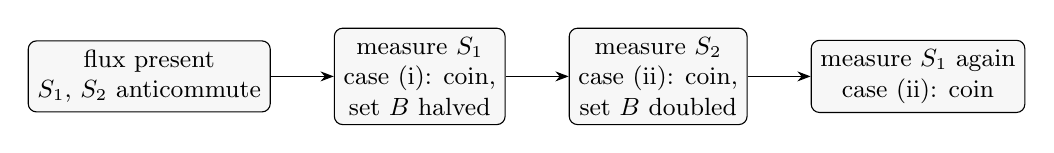
\begin{tikzpicture}[font=\small, box/.style={draw, rounded corners=3pt, minimum height=8mm, align=center, fill=gray!6}]
  \node[box] (s0) {flux present\\ $S_1$, $S_2$ anticommute};
  \node[box, right=8mm of s0] (s1) {measure $S_1$\\ case (i): coin,\\ set $B$ halved};
  \node[box, right=8mm of s1] (s2) {measure $S_2$\\ case (ii): coin,\\ set $B$ doubled};
  \node[box, right=8mm of s2] (s3) {measure $S_1$ again\\ case (ii): coin};
  \draw[-{Stealth}] (s0) -- (s1);
  \draw[-{Stealth}] (s1) -- (s2);
  \draw[-{Stealth}] (s2) -- (s3);
\end{tikzpicture}
\caption{Re-randomisation while a flux survives. The second outcome of $S_1$ agrees with the first only with probability $\tfrac12$.}
\label{fig:aba}
\end{figure}

\subsection{One shot}
\begin{enumerate}
\item Start: $x=0$, $B=C_0$, $Q=0$; an equal superposition of the eight logical (winding) sectors of the three colours.
\item Every round: noise (updates $x$ and $Q$) $\to$ $Z$-type checks (read from $x$) $\to$ real-time flux correction (updates $x$) $\to$ dressed checks colour by colour (Sec.~4.1).
\item End: close the remaining fluxes, remove $x$ by applying products of checks, and measure one perfect round. Without fluxes all checks commute, so the state is now a code state times charges.
\item Logical fidelity: for each of the eight sectors, read whether it lies in $B$ and the value of $Q$, and compute the overlap with the initial state as an \emph{exact number}, not a sample.
\end{enumerate}

\section{Cost}

The linear system for $B$ and the form $Q$ are binary matrices of size at most $k\times k$ ($k=3L^2$), stored 64 bits to a word. A measurement costs $O(k^2)$ bit operations; at $L=9$ ($k=243$) a matrix occupies about 7\,kB. Measured cost per shot (phenomenological noise at $p=2\%$, decoding included, one process):
\begin{center}
\begin{tabular}{rrrrp{0.3\linewidth}}
\toprule
$L$ & qubits & \shortstack{twisted frame\\(production)} & \shortstack{Pauli proxy\\(same task)} & dense state vector \\
\midrule
3 & 81 & 0.33\,ms & 4.1\,ms & $2^{27}$ amplitudes; 0.1--1\,s per shot on a GPU \\
5 & 225 & 0.89\,ms & 18\,ms & impossible ($2^{75}$) \\
7 & 441 & 2.2\,ms & 79\,ms & impossible \\
9 & 729 & 6.3\,ms & 236\,ms & impossible \\
\bottomrule
\end{tabular}
\end{center}
The Pauli-proxy column is a per-shot Python implementation; driven by the same per-shot code, it is $3.5$--$6.8$ times slower than the twisted frame, and $37$ times slower than the batched production engine at $L=9$ (the latter ratio also includes implementation differences).

\section{How we know it is right}
\begin{itemize}
\item \textbf{Proof.} The Proposition above (proved in the study-1 manuscript).
\item \textbf{Dense state vector at $L=3$.} Driven by the same noise, a brute-force simulation that applies every operation literally (in the circuit-level model every CNOT and CCZ) gives the same outcome probabilities (to $<10^{-6}$) and the same final fidelities.
\item \textbf{Independent method at $L=3$--$9$.} A separate implementation of the Pauli-proxy method of Takada, Bartlett and Williamson agrees on 14\,400 trajectories (about $5.3\times10^6$ measurements, $4.2\times10^5$ of them random) exactly.
\item \textbf{Negative control.} Removing the Pauli dressing (the term $q(b+s+x)+q(b+s)$ in Eq.~\eqref{eq:f}) breaks the agreement within the first trajectories.
\end{itemize}

\section{Why it applies to study 1, and why we should use it}

\subsection{The assumptions hold}
\begin{center}
\begin{tabular}{>{\raggedright}p{0.44\linewidth}p{0.48\linewidth}}
\toprule
assumption of the Proposition & situation in study 1 \\
\midrule
the initial state is an error-free code state (so Eq.~\eqref{eq:identity} holds) & the memory experiment starts from the code state \\
the noise consists of Pauli errors & true for the phenomenological, code-capacity and circuit-level Pauli models \\
only Pauli operators, CZ gates, $Z$-type checks and dressed checks (possibly times $Z$) occur & true for the memory experiment; in the circuit-level model a Pauli fault propagated through the CNOT/CCZ circuit becomes a Pauli times CZ gates, and a faulty measurement becomes a projection followed by Pauli and CZ errors (checked against the fault tables) \\
the state stays on flat configurations & $X$ errors are kept in $x$, so $B$ is always flat \\
the structure of the $\mathbb{D}_4$ code (quadratic CZ part, check shifts inside $C_0$) & it is the $\mathbb{D}_4$ code \\
\bottomrule
\end{tabular}
\end{center}

\subsection{Reasons to use it}
\begin{enumerate}
\item \textbf{No approximation.} The re-randomisation by non-commuting checks and the CZ-type residues, which the previous surrogate could not represent, are included automatically. The conclusions of study~1 (crossings near $2\%$, below the earlier $2.4\%$) rely on this.
\item \textbf{Speed.} About 6\,ms per shot at $L=9$, so the production run ($10^5$ shots $\times$ 10 points $\times$ 4 sizes $\times$ 3 variants) fits into 10--15 hours on one Colab machine, and $L=11$ is within reach. The dense state vector stops at $L=3$, and the general Pauli-proxy method is several to tens of times slower for the same task.
\item \textbf{Exact numbers, not only samples.} Whether each outcome was random and the final logical fidelity (including values strictly between $0$ and $1$) are available exactly, which also yields precise diagnostics such as the fraction of random outcomes in flux-free layers.
\item \textbf{An independent cross-check.} It shares no state representation with the Pauli-proxy method used in studies~2 and~3, so their agreement is strong evidence for both.
\end{enumerate}

\subsection{When not to use it}
\begin{itemize}
\item Protocols with a logical non-Clifford gate such as the switching unitary $U$ (studies 2 and 3 use the Pauli-proxy method).
\item Patches with boundaries: the principle is the same, but the implementation is for the torus.
\item Non-Pauli (coherent) noise, or faults inside a $T$-gate decomposition of the CCZ gate.
\item Other codes: the method relies on flat configurations and a cubic sign. At higher levels of the hierarchy (study 5, $N\ge4$) the checks contain CCZ gates and the form is not preserved.
\end{itemize}

\section{Relation to the method of Takada, Bartlett and Williamson}
Their Clifford-stabilizer simulation tracks groups of stabilizers that may not commute as operators but commute on the stabilized subspace. The twisted frame is a \emph{special case}:
\begin{itemize}
\item the commutator of two dressed checks is a product of $Z$-type checks, so each measurement is effectively commuting or anticommuting and its outcome is certain or a fair coin (their Sec.~VI.A);
\item case (ii) is their update rule for anticommuting measurements (Secs.~IV and VI.B), written for the state;
\item the term $q(b+s+x)+q(b+s)$ is their Pauli dressing.
\end{itemize}
The difference is what is stored. Their method keeps a Pauli-stabilizer tableau of a proxy state in which non-Pauli factors are replaced by Pauli ones; it applies to any code that meets its conditions. The twisted frame uses the structure of the $\mathbb{D}_4$ code to store the support and signs of the true state directly; it is specific to this code, gives amplitude information directly, and is faster.

The name \emph{twisted frame} is not an established term but was introduced in this project; in the paper it should be introduced as ``we call this representation the \emph{twisted frame}''.

\end{document}
